\chapter{Biomedical concept disambiguation}
\label{c3}

In natural language text it is frequent that words or phrases\footnote{In this context, a phrase is considered a group of words that forms a grammatical unit, playing a specific role within the syntactic structure of a sentence. \url{https://en.wikipedia.org/wiki/Phrase}} are ambiguous, that is, they can convey different meanings depending on the surrounding context.
As stated by \textcite{navigli2009a}, identifying the correct sense of an ambiguous word in a specific context is only apparently simple---while humans generally do not even notice the ambiguities of language, machines need to process \textit{unstructured text} and extract structured information to determine the underlying meaning.

In detail, as \textcite{vicente2017a} explain, a \textit{monosemous} term has only one meaning, and terms with multiple senses can be considered \textit{polysemous} or \textit{homonymous}.
\textit{Polysemous} terms are associated with two or more related senses, whereas in contrast \textit{homonymous} terms are associated with two or more unrelated meanings.
These phenomena are denominated as \textit{monosemy}, \textit{polysemy} and \textit{homonymy}.
In this work, to simplify the task at hand, we make no distinction between \textit{polysemous} and \textit{homonymous} terms, henceforward referring to them as ambiguous terms.
However, we stress that tackling \textit{polysemy} and \textit{homonymy} separately has the potential to improve downstream \as{nlp} (natural language processing) tasks.
For instance, \textcite{krovetz1997a} has demonstrated its value in information retrieval.

The computational identification of the correct meaning of an ambiguous word (or term) given a specific context is known as word sense disambiguation (\as{wsd}), and it is considered an \as{ai}-complete problem relevant for natural language understanding \parencite{navigli2009a,ide1998a}.
This is an important task for extracting accurate information from text.
Generally, the first major step in information extraction is \textit{concept recognition} which is responsible for identifying concepts of specific classes, such as chemicals or diseases, in the text.
This task can be articulated as a pipeline of two subtasks: (1)~named entity recognition (\as{ner}) followed by (2)~disambiguation and normalization  (\Cref{fig:nern}).

% \FloatBarrier
\begin{figure}[!tb]
\begin{center}
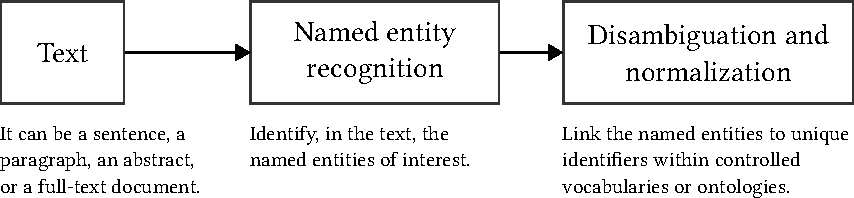
\includegraphics[width=\textwidth]{img/nern/v4/img.pdf}
\caption{Named entity recognition and normalization pipeline.}
\label{fig:nern}
\end{center}
\end{figure}
% \FloatBarrier


The aim of \as{ner} is to identify the text spans mentioning concepts of specific types. However, the sole utility of \as{ner} is limited because detected named entities are not linked to controlled vocabularies or ontologies, which is required for many end-user tasks \parencite{leaman2016b}.
Named entity normalization, or named entity linking, is the process of associating detected named entities with unique identifiers from standard knowledge bases.
Undoubtedly, this is entwined with disambiguation: often, named entities convey multiple meanings that are associated with several unique identifiers.
In this case, disambiguation methods are applied to each ambiguous named entity for selecting the correct unique identifier, amongst a set of candidate unique identifiers, according to its surrounding context.
The \textit{concept recognition} task is considered to be completed after the entity mentions are identified and linked to established databases.
\Cref{fig:chemical-entity-annotations} provides an example text with chemical concepts annotated and linked within the \as{mesh} (Medical Subject Headings) vocabulary.

% \FloatBarrier
\begin{figure}[!tb]
\begin{center}
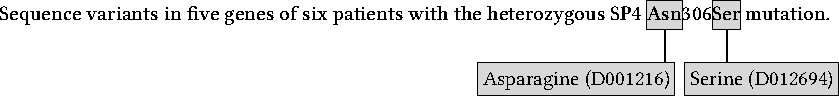
\includegraphics[width=\textwidth]{img/chemical-entity-annotations/v1/img.pdf}
\caption[Example text with chemical entity annotations.]{Example text with chemical entity annotations. Annotations from the \as{pmid} 17356515 document in the NLM-Chem dataset \parencite{islamaj2021a}. The outer boxes contain the associated \as{mesh} heading and unique identifier.}
\label{fig:chemical-entity-annotations}
\end{center}
\end{figure}
% \FloatBarrier


This chapter is mainly focused on disambiguation, but work on entity normalization is also  discussed.
We summarize related work, detail common resources for assessing these tasks, and describe our solutions.
Based on distributed representations of words, or simply \textit{word embeddings}, we propose supervised learning and knowledge-based approaches for biomedical \as{wsd}, and a method for normalization of clinical terms.


\section{Background}

For a long time, word sense disambiguation has been a challenging problem in computational linguistics, and even its definition has been a topic of debate.
\textcite{kilgarriff1997a} dicusses the concept of \textit{word senses} arguing that word senses only exist relative to a specific task.
The author further extends this discussion gathering evidence from lexicographers and philosophers, stating that word senses are not easy to inventorize \parencite{kilgarriff2007a}.

\textcite{ide1998a} present an exhaustive review about \as{wsd} putting into perspective the past work on the topic since around the 1950s.
The authors make a survey of several methods (knowledge-based and corpus-based), discuss several aspects and issues including the role of context, the disagreement on sense divisions, and the difficulty of evaluation and comparison of systems.
Some of the first approaches for sense disambiguation relied on machine-readable dictionaries \parencite{lesk1986a,veronis1990a} with particular emphasis for improving information retrieval systems \parencite{krovetz1989a}.
\textcite{sanderson1994a,sanderson1996a} also extensively explored the impact of lexical ambiguity and disambiguation on information retrieval, concluding that very small queries benefit most from disambiguation than other queries that contain a sufficient number of words and provide enough context to implicity resolve ambiguities.
\textcite{yarowsky1995a} proposed an unsupervised learning algorithm for sense disambiguation that matched the performance of supervised techniques, arguing that the cost of annotating a large training corpus may not be necessary to achieve a good \as{wsd} performance.
\textcite{stevenson2001a} showed that combining different knowledge sources can further improve \as{wsd}, and proposed a sense tagger that surpassed an accuracy of 94\% on their evaluation corpus.

WordNet~\parencite{fellbaum1998a,miller1995a} is a large lexical database of the English language, created at Princeton University, that has been extensively used for tackling \as{wsd} in the general domain \parencite{banerjee2002a,loureiro2019a}.
It comprises synonyms that are grouped into unordered sets (synsets), each containing a brief definition and, in most cases, sample sentences showing its use.
Despite its large coverage for general-domain concepts, other specific-domains---such as the life sciences field---require specialized thesauri and vocabularies.
Presumably, the most used lexical database in the biomedical sciences is the Unified Medical Language System (\as{umls}), comprising many controlled vocabularies, and a comprehensive thesaurus and semantic network of biomedical concepts \parencite{bodenreider2004a}.
For instance, it includes clinical terminologies such as \as{snomed} CT (Systematized Nomenclature of Medicine Clinical Terms), \as{loinc} (Logical Observation Identifiers Names and Codes), and RxNorm \parencite{bodenreider2018a}.
Besides these, many other biomedical ontologies and controlled vocabularies exist, but some are specific for a certain class of biomedical concepts such as drugs or diseases.
For example, the \as{mesh} vocabulary is used to index \as{pubmed} articles which facilitates searching for topics of interest \parencite{lipscomb2000a}.

Much of the research work in \as{wsd} and entity linking has been developed within the general-domain, but in this thesis we focus on the extraction of knowledge from biomedical text and are interested in the application of these tasks in free text from life-sciences scientific literature and clinical records.
Thus, henceforward, we will focus here on reviewing prior work on biomedical entity disambiguation and normalization, since they have long been considered fundamental tasks for biomedical text mining \parencite{schuemie2005a,krauthammer2004a}.

Traditionally, external sources of information such as \as{umls} serve to fuel \as{wsd} knowledge-based methods that are employed in an unsupervised fashion and do not require labeled training data \parencite{jimenoyepes2010a,mcinnes2011a,elrab2013a,garla2013a,mcinnes2013a,duque2018a}.
Nonetheless, supervised or semi-supervised methods, based on machine learning, may not use external knowledge and still perform better due to having access to labeled training data \parencite{mcinnes2014a,jimenoyepes2017a}.
The difference between supervised and semi-supervised methods is in the quality of labeled training data.
Supervised learning makes use of \textit{ground-truth} or \textit{gold-standard} training data that is annotated by domain experts.
Such models produce less realistic results since the creation of gold-standard training data is very expensive, limited, and may be considered insufficient for obtaining a well-trained supervised model able to generalize to unseen data.
Due to the problem of limited annotation human power, semi-supervised, and \textit{weak} or \textit{distant} supervision strategies have been investigated \parencite{li2019f}.
These make use of \textit{silver standard} training data that are created (1)~through heuristics or handcrafted rules, or (2)~by using existing knowledge from common databases.
Recent approaches have been using external resources to build concept embeddings \parencite{sabbir2016a,newmangriffis2018a}.
And, as shown by \textcite{tsai2016a,siu2016a}, the use of multiple knowledge databases also brings benefits to the problem of biomedical concept disambiguation.


\section{Available corpora}

\begingroup
% \normalfont
% \color{black}

\newcommand{\z}{\hspace*{1em}}
\newcommand{\minorsmall}{\fontsize{10.5pt}{12.6pt}\selectfont}
\newcommand{\minorfootnotesize}{\fontsize{9.7pt}{11.64pt}\selectfont}

\begin{table}[!tb]

\caption[Datasets for biomedical word sense disambiguation.]{Datasets for biomedical word sense disambiguation, presented in chronological order. MSH: Medical Subject Headings. NLM: National Library of Medicine. UMLS: Unified Medical Language System. UMN: University of Minnesota. VUH: Vanderbilt University Hospital. WSD: word sense disambiguation.}
\label{tab:wsd-datasets}

\centering

\begin{tabular}{E{0.30\textwidth}p{0.62\textwidth}}

\toprule

% \textbf{Resource} & \textbf{Description}\\
Resource & Description\\

\midrule

NLM WSD test collection\newline
\z{\minorsmall\parencite{weeber2001a}}
&
A collection comprising 50~ambiguous terms with a total of 5000 disambiguated instances. Abstracts from the 1998 MEDLINE citations were used. The terms were mapped to the 1999 version of the UMLS.\newline
{\minorfootnotesize\url{https://lhncbc.nlm.nih.gov/ii/areas/WSD/original.html}}
\\

\midrule

MSH WSD dataset\newline
\z{\minorsmall\parencite{jimenoyepes2011a}}
&
A dataset containing 203 ambiguous terms with a total of 37\,888 ambiguity instances retrieved from the 2010 MEDLINE. The 2009AB UMLS version was used to map the terms.\newline
{\minorfootnotesize\url{https://lhncbc.nlm.nih.gov/ii/areas/WSD/collaboration.html}}
\\

\midrule

VUH admission notes\newline
\z{\minorsmall\parencite{wu2013a,wu2015a}}\newline
\z{\minorsmall\parencite{wang2016b,wang2018j}}
&
It contains 25 ambiguous abbreviations, from clinical admission notes, with up to 200 sentences containing each abbreviation. These were randomly selected and manually annotated by experts.
\\

\midrule

UMN clinical notes\newline
\z{\minorsmall\parencite{moon2014a}}\newline
\z{\minorsmall\parencite{wu2015a}}\newline
\z{\minorsmall\parencite{wang2016b}}
&
A dataset containing 75 acronyms and abbreviations (short forms) with their possible senses (long forms). Senses of each ambiguous term were manually annotated from 500 random instances and matched with the 2011AB UMLS version.\newline
{\minorfootnotesize\url{https://hdl.handle.net/11299/137703}}
\\

\bottomrule

\end{tabular}
\end{table}
\endgroup


\begingroup
% \normalfont
% \color{black}

\newcommand{\z}{\hspace*{1em}}

\begin{table}[!tb]

\caption[Datasets for biomedical named entity normalization.]{Datasets for biomedical named entity normalization, presented in chronological order. CDR: chemical disease relation. CUI: Concept Unique Identifier. MCN: Medical Concept Normalization. MeSH: Medical Subject Headings. NCBI: National Center for Biotechnology Information. NLM: National Library of Medicine. OMIM: Online Mendelian Inheritance in Man. PMC: PubMed Central. ShARe: Shared Annotated Resources. UMLS: Unified Medical Language System.}
\label{tab:nen-datasets}

\centering

\begin{tabular}{E{0.30\textwidth}p{0.62\textwidth}}

\toprule

% \textbf{Resource} & \textbf{Description}\\
Resource & Description\\

\midrule

NCBI disease corpus\newline
\z{\small\parencite{dogan2012a}}\newline
\z{\small\parencite{leaman2013a}}\newline
\z{\small\parencite{dogan2014a}}
& A collection of 793 \as{pubmed} abstracts containing disease entity mentions and their corresponding \as{mesh} or \as{omim} identifiers, where each abstract was manually annotated by two experts. A total of 6982 disease mentions are mapped to 790 unique identifiers.\newline
{\footnotesize\url{https://www.ncbi.nlm.nih.gov/CBBresearch/Dogan/DISEASE}}
\\

\midrule

ShARe corpus\newline
\z{\small\parencite{elhadad2015a}}\newline
\z{\small\parencite{pradhan2015a}}
& The SemEval-2015 ShARe corpus is comprised of 531 de-identified clinical notes (discharge summaries and radilogy reports) annotated with disorder mentions along with their normalization to the \as{umls} terminology using \asp{cui}.\newline
{\footnotesize\url{http://share.healthnlp.org}}
\\

\midrule

BC5CDR corpus\newline
\z{\small\parencite{li2015a,li2016b}}
& It contains 1500 \as{pubmed} abstracts annotated with biomedical entity mentions linked with \as{mesh} identifiers, with a total of 4409 chemicals and 5818 diseases.\newline
{\footnotesize\url{https://biocreative.bioinformatics.udel.edu/tasks/biocreative-v/track-3-cdr}}
\\

\midrule

MCN corpus\newline
\z{\small\parencite{luo2019a,luo2020b}}
&
A wide-coverage corpus for clinical concept normalization including annotated medical problems, treatments, and tests. It consists of 100 discharge summaries with a total of 10\,919 concept mentions mapped to 3792 unique identifiers from two controlled vocabularies---RxNorm \parencite{liu2005a,nelson2011a} and \as{snomed} CT \parencite{cote1986a,stearns2001a,cornet2008a,bodenreider2018a}.\newline
{\footnotesize\url{https://n2c2.dbmi.hms.harvard.edu/2019-track-3}}
\\

\midrule

NLM-Chem corpus\newline
\z{\small\parencite{islamaj2021a,islamaj2021c}}
& It consists of 150 full-text \as{pmc} articles, doubly annotated by ten \as{nlm} experts, with a total of 38\,942 chemical entity mentions, which correspond to 4867 unique chemical names and 2064 \as{mesh} identifiers.\newline
{\footnotesize\url{https://biocreative.bioinformatics.udel.edu/tasks/biocreative-vii/track-2}}
\\

\bottomrule

\end{tabular}
\end{table}
\endgroup


In this section, for conciseness, we only present available research corpora---datasets used for common and standard evaluation---employed for the specific tasks regarding biomedical word sense disambiguation and entity normalization.
However, for more biomedical \as{nlp} resources that are frequently adopted for solving these tasks, we point the reader to \Cref{c2:s:biomedical-text-mining} where we present some of the most well-known external knowledge sources, and additionally enumerate \as{nlp} competitions or shared tasks that addressed, and have been fostering, the development of solutions for biomedical concept disambiguation.

Annotated datasets are required to evaluate automatic systems, but manual curation by domain experts is an expensive and cumbersome task that is often not enough \parencite{baumgartner2007a,howe2008a,karp2016a}.
It is therefore of utmost relevance to publicly share such resources for research purposes to further the development and improvement of these text mining methods.

\Cref{tab:wsd-datasets} presents some of the most well-known datasets for evaluating biomedical \as{wsd} systems.
In our work, we use the MSH WSD dataset since it is one of the most used, and largest, datasets for evaluating \as{wsd} in biomedical scientific literature \parencite{jimenoyepes2011a}.
Similarly, \Cref{tab:nen-datasets} presents some of the standard datasets for biomedical named entity normalization.
For this task, we use the \as{mcn} (Medical Concept Normalization) corpus \parencite{luo2019a} for assessing our knowledge-based normalization method in the clinical domain.


\section{Biomedical word sense disambiguation}

In this section we present our studies about biomedical \as{wsd} methods.
At first, we describe our research about the impact of using general-domain \versus\ domain-specific embedding models for disambiguation of ambiguous terms in biomedical scientific abstracts \parencite{antunes2016a}.
Then, we present an exhaustive study of different methods for tackling biomedical \as{wsd} \parencite{antunes2017a,antunes2017b,antunes2017c}.
We compare the use of traditional text feature engineering (bag-of-words) against the use of word embeddings using a plethora of machine learning classifiers.
We propose a knowledge-based method based on word embeddings, concept textual definitions, and concept associations---derived from \as{mesh} term co-occurrences---that achieves competitive results.
We also investigate the impact of using different word embeddings averaging functions according to the distance between the ambiguous term and the remaining words of the surrounding context.
In all these works we used the MSH WSD dataset for evaluation of our methods.


\subsection{MSH WSD dataset}

The MSH WSD dataset is likely the most used resource for evaluating biomedical \as{wsd} systems.
It was generated by an automatic method proposed by \textcite{jimenoyepes2011a}, using the \as{umls} Metathesaurus and the manual \as{mesh} indexing in \as{medline} citations.
The data consists of \as{pubmed} scientific abstracts, each with one ambiguous term identified and mapped to the correct sense using \as{umls} Concept Unique Identifiers (\asp{cui}).
It contains 203 ambiguous terms (88 are regular terms, 106 are abbreviations, and 9 are a mix of both) with a total of 423 distinct senses.
Most of the terms (189) have only two different meanings, 12 terms have three different meanings, and the remaining 2 terms have four and five different meanings.
For each possible sense there is a maximum of 100 instances, that is, abstracts where the ambiguous term occurs.
There are a total of 37\,888 examples of ambiguity, and each term has on average 187 ambiguity cases.


\subsection{General-domain \versus\ domain-specific word embeddings}
\label{c3:ss:general-vs-specific}

In this section we present our experiments with traditional machine learning classifiers for evaluating the impact of using general-domain and domain-specific (biomedical) word embeddings models for biomedical \as{wsd} \parencite{antunes2016a}.


\subsubsection{Methodology}

In order to get a greater judgment of the performance of the two word embeddings models, we employed several machine learning classifiers using the scikit-learn framework\footnote{For details about these classifiers we point the reader to the scikit-learn web page: \url{https://scikit-learn.org}.} \parencite{pedregosa2011a}: decision tree, k-nearest neighbors, passive aggressive linear model, ridge regression, and two different implementations of support vector machines.
For a fair evaluation, we applied 5-fold cross-validation to split the abstracts set, of each ambiguous term, in training and test subsets.
A list of 313 stop words obtained from the \as{medline} repository\footnote{\url{https://data.lhncbc.nlm.nih.gov/public/ii/information/MBR/WordCounts/2009/wrd_stop}} was used to filter out less relevant words in the corpus.


\paragraph{Word embeddings}

Two word embeddings models were created: one for the general-domain and another specific to the biomedical domain using textual data from Wikipedia and \as{pubmed}, respectively.
Wikipedia is range-wide having no specific domain.
We used the full Wikipedia dump, obtained in September 2015, amounting to approximately four million articles and containing about two million distinct words.
On the other hand, \as{pubmed} is specific to the biomedical domain.
Around six million abstracts corresponding to the years 2010 to 2015 were used, containing around 400~thousand distinct words.
Both models were trained with the Gensim framework \parencite{rehurek2010a} using a window of five words and for a feature vector of size 100.
Each abstract was represented by the weighted average of the vector embeddings of the respective words, with the \as{tf}--\as{idf} value of each word used as weight.


\subsubsection{Results and discussion}

\Cref{tab:wsd-wikipedia-vs-pubmed} presents the macro-accuracy results using several machine learning classifiers and two different word embeddings models (Wikipedia and \as{pubmed}).
The model specific to the biomedical domain---created with \as{pubmed} abstracts---consistently outperformed the general model created from Wikipedia articles.
Nevertheless, the results obtained with the latter indicate that even features extracted from general-domain corpora may contribute to these methods.
The highest accuracy result using the Wikipedia model (support vector classification) exceeds the lowest accuracy result using the \as{pubmed} model (decision tree) by around 6 percentage points (0.912 \vs\ 0.849), which demonstrates that the selection of an appropriate classifier is also important.
The highest accuracy result obtained was 0.928 corresponding to the use of the word embeddings model from \as{pubmed} and the application of the passive aggressive classifier.

\begingroup
% \normalfont
% \color{black}

\begin{table}[!tb]

\caption[Accuracy disambiguation results, in the MSH WSD dataset, using different machine learning classifiers and word embeddings from the general and biomedical domains (Wikipedia and \as{pubmed}).]{Accuracy disambiguation results, in the MSH WSD dataset, using different machine learning classifiers and word embeddings from the general and biomedical domains (Wikipedia and \as{pubmed}). Results shown are the average across five folds. DT: decision tree; kNN: k-nearest neighbor (k=5); PA: passive aggressive linear model; RR: ridge regression; SGD: linear support vector machine with stochastic gradient descent; SVC: support vector classification.}
\label{tab:wsd-wikipedia-vs-pubmed}

\centering

\large

\begin{tabular}{E{20mm}T{36mm}T{30mm}}

\toprule

Classifier & \multicolumn{2}{c}{Model of word embeddings from}\\

% \cmidrule(r){1-1}\cmidrule(l){2-3}
% \midrule

% & \textbf{Wikipedia} & \textbf{PubMed}\\
& Wikipedia & PubMed\\

\cmidrule(r){1-1}\cmidrule(l){2-3}

DT  & 0.817 & 0.849\\
kNN & 0.896 & 0.918\\
PA  & 0.893 & \textbf{0.928}\\
RR  & 0.905 & 0.910\\
SGD & 0.874 & 0.916\\
SVC & \textbf{0.912} & 0.924\\

\bottomrule

\end{tabular}
\end{table}
\endgroup



\subsection{Supervised learning and knowledge-based methods}
\label{c3:ss:supervised-and-kb}

In this section, we present an exhaustive study of supervised learning and knowledge-based methods for biomedical \as{wsd} \parencite{antunes2017c}.
We describe our knowledge-based method and evaluate the impact of using different word vector embeddings averaging functions for representing the surrounding context of ambiguous terms \parencite{antunes2017a,antunes2017b}.


\subsubsection{Implementation}

Supervised learning and knowledge-based methods are applied to the MSH WSD dataset in order to measure and compare the accuracy results of disambiguation.
Bag-of-words features are used only in the supervised setting whereas word embeddings---created with unlabeled \as{medline} abstracts---are used in both approaches.
From the \as{umls} Metathesaurus we extracted \as{cui} textual definitions to be used in the knowledge-based approach.
The word embeddings are used to calculate vector embeddings for: (1)~the surrounding contexts of the ambiguous terms, henceforward denoted as context embeddings or context vectors; and (2)~\as{cui} textual definitions extracted from \as{umls}, henceforward denoted as concept embeddings or concept vectors.
The knowledge-based method finds the most likely sense for a specific ambiguous term by evaluating the similarity between its context vector and all the concept vectors weighted by \as{cui}--\as{cui} association values.
Each step is described in detail in the following paragraphs.


\paragraph{Word embeddings}

The word embeddings models were generated using \as{pubmed} articles which are specific to the biomedical domain.
\as{medline} abstracts corresponding to the years 1900 to 2015 were used, containing around 15~million documents with a total of around 800~thousand unique words.
We trained six word embeddings models using context windows of 5, 20, and 50 words, and vector sizes of 100 and 300.
For generating the word embeddings vectors we used the continuous bag-of-words model proposed by \textcite{mikolov2013b}, implemented in the Gensim framework \parencite{rehurek2010a}.
The word embeddings are used to calculate the context embeddings and the concept embeddings as explained next.


\paragraph{Context embeddings}

The context embeddings are vectors that represent the surrounding contexts of the ambiguous terms.
We consider the surrounding context of an ambiguous term to be all the words of the respective document excluding the ambiguous term occurrences.
Each context vector is obtained by weighting the vector embeddings of the respective words using different weighting schemes.
In the end, all the context vectors are normalized (L2 norm equal to 1).

In the supervised learning setting we considered the \as{tf}--\as{idf} weighting scheme, whereas in the knowledge-based method we additionally tested four averaging functions which consisted of word distance decay functions multiplied by the \as{idf} value.
The objective of using decay functions, instead of the term frequency component, was to give greater importance to closest words of the ambiguous term, since we hypothesized that the nearest words to the ambiguous term may be more relevant for disambiguation.
The absolute word distance $d$ between some specific word and the closest occurrence of an ambiguous term was defined as being the input variable of the decay function.
The five weighting schemes, with the \as{idf} value being used as a multiplicative factor, were:

\begin{itemize}
\item
Term frequency;
\item
No decay (constant): $\functionf(d) = 1$;
\item
Fractional decay: $\functionf(d) = 1 / d$;
\item
Exponential decay: $\functionf(d) = \exp(-d)$;
\item
Logarithmic decay: $\functionf(d) = 1 / \ln{\left(1 + d\right)}$.
\end{itemize}


\paragraph{Concept embeddings}

The concept embeddings are only relevant to the knowledge-based method.
We extracted, from \as{umls} knowledge sources\footnote{\url{https://www.nlm.nih.gov/research/umls/licensedcontent/umlsknowledgesources.html}}, textual definitions for every \as{cui} which were used to create the concepts vector embeddings---the \as{tf}--\as{idf} value was used to weight the word vectors.
Alike the context embeddings, all the vectors were normalized.


\paragraph{CUI--CUI association values}

We calculated \as{cui}--\as{cui} association values as normalized pointwise mutual information (\as{npmi})\footnote{\url{https://en.wikipedia.org/wiki/Pointwise_mutual_information}} from the \as{mesh} co-occurrence counts in \as{medline} citations\footnote{Since the MSH WSD dataset uses \asp{cui} to identify the distinct term senses, we used the \as{mesh} to \as{cui} mapping in \as{umls} to translate the \as{mesh} term associations to \as{umls} concept--concept associations.}\textsuperscript{,}\footnote{\url{https://ii.nlm.nih.gov/MRCOC.shtml}}.
A \as{npmi} value is between -1 and 1, with -1 for never occurring together, 0 representing independence, and 1 a complete association (a concept in relation to itself has a value of 1).
Since there is a large number of \asp{cui}, and consequently the number of possible \as{cui}--\as{cui} associations is much higher, we kept only the association values with \as{npmi} values greater or equal than 0.3.
These are only used in the knowledge-based method.


\paragraph{Supervised learning classification}

We tested five machine learning classifiers from the scikit-learn framework \parencite{pedregosa2011a}: decision tree, k-nearest neighbors, logistic regression, multi-layer perceptron, and support vector machine.
Bag-of-words, containing unigrams and bigrams weighted by \as{tf}--\as{idf}, and context embeddings were used as input features to train the classifiers.
For each ambiguous term, 5-fold cross-validation was used to split the corresponding abstracts set for training and testing the classification models.


\paragraph{Knowledge-based method}

The knowledge-based method does not require training from the target dataset, being only dependent on knowledge from external sources.
Our method relies on the idea of comparing the surrounding contexts of the ambiguous terms with the concepts' textual definitions---the aim is to find the most similar concept (likely meaning) given a specific context.

As described earlier, each \as{cui} was represented by a concept vector, and the surrounding context of an ambiguous term was represented by a context vector.
Therefore, it is straightforward to infer the most related sense of an ambiguous term by calculating the cosine similarity between the context vector and each \as{cui} vector, and selecting the most similar one. \Cref{fig:context-vector-spatial-representation} illustrates a visual example.

% \FloatBarrier
\begin{figure}[!tb]
\begin{center}
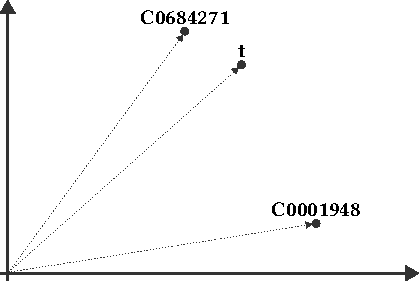
\includegraphics[width=0.6\textwidth]{img/context-vector-spatial-representation/v5/img.pdf}
\caption[Exemplificative spatial representation of the context vector of an ambiguous term.]{Exemplificative spatial representation of the context vector of an ambiguous term and the vectors of two candidate \asp{cui}. In this example, one can visualize that the closest concept vector to the context~$\tvec$ is relative to the C0684271 identifier which would be the one selected as the correct meaning.}
\label{fig:context-vector-spatial-representation}
\end{center}
\end{figure}
% \FloatBarrier


We extended this baseline approach by calculating a score for each candidate \as{cui} of an ambiguous term, and the \as{cui} with highest score is selected as the correct meaning.
The score is obtained using the cosine similarities between the context vector and every concept vector weighted by \as{cui}--\as{cui} association values (one concept is the candidate sense, and the other is the one whose textual definition is being compared with the context).
The intuition behind this idea is that if a distinct concept has a strong association with the candidate concept, and its textual definition is similar to the context in which the ambiguous term is inserted, then the likelihood of the respective candidate \as{cui} to be the correct sense must be increased (likewise, if the association is weak then the likelihood must be decreased).
The score function is defined in \Cref{eq:kb-score}.

\begin{equation}
\label{eq:kb-score}
\score(\CUI) = \frac{1}{N} \sum\limits_{j}{} \NPMI(\CUI, \CUI_j) \cdot \CS(\tvec, \CUIvec_j)
\end{equation}

According to \Cref{eq:kb-score}: the $\CUI$ variable represents a candidate meaning; the $\CUI_j$ variable represents any other related concept; the $\tvec$ variable corresponds to the context vector; and $\CUIvec_j$ is the concept vector of the related concept $\CUI_j$.
The context $\tvec$ of a specific candidate is compared to every concept textual definition $\CUIvec_j$ by its cosine similarity $\CS(\tvec, \CUIvec_j)$, which is then weighted by the $\NPMI(\CUI, \CUI_j)$ association value.
The $N$ variable is the total number of associations considered, corresponding to the number of $\NPMI$ values, and it is used to normalize the final score.
For each candidate $\CUI$---from a set of possible concepts, given a specific ambiguous term---a score is calculated, and the one that obtains the highest score is considered as the correct sense.


\subsubsection{Results and discussion}

In both approaches, supervised and knowledge-based, the dataset was split into five folds, and the final results were obtained by averaging the results of each fold.
\Cref{tab:wsd-supervised} and \Cref{tab:wsd-kb} present the disambiguation accuracy results obtained by the supervised machine learning classifiers and the knowledge-based method respectively.

Regarding the supervised learning setting, the highest accuracy (0.9557) was obtained combining unigrams and word embeddings features using a multi-layer perceptron.
However, the best result using only bag-of-words features---unigrams and bigrams---is very close (0.9552) and was achieved by a support vector machine, showing that the state-of-the-art results for this problem can be reproduced using simple word-based features.
Similarly, the sole use of word embeddings features with the multi-layer perceptron attained a close performance (0.9514).
We observe that the performance variations using distinct word embeddings models trained with different vector sizes (100 and 300) and context windows (5, 20, and 50) are not significant\footnote{Using different dataset splits or random seeds for initializing model parameters would likely produce small variations in the results.}, concluding that any of these models perform reasonably well.
It is also noticeable that the use of bigrams contribute only slightly to the results, and unigram features alone achieve almost as good if not better results than the combination of unigrams and bigrams.
Finally, we note that the decision tree model obtained the lowest results, below around 2--3 percentage points overall, in comparison to the other four classifiers.
Remarkably, the k-nearest neighbors, a simple baseline model, achieved consistent and competitive performances with different combinations of features---attaining a top accuracy of 0.9475---which indicates that the features in use provide effective text representations.

\begingroup
\newcommand{\z}{\hphantom{0}}

\begin{table}[!tb]

\caption%
[Supervised learning disambiguation results in the MSH WSD dataset using bag-of-words and word embeddings features.]%
{Supervised learning disambiguation results in the MSH WSD dataset using bag-of-words and word embeddings features. The evaluation metric is accuracy and the results were obtained using 5-fold cross-validation. Rows 1--3 present the results using only bag-of-words features (unigrams, bigrams, and both), rows 4--9 present the results using only word embeddings (different vector sizes and windows), and rows 10--15 present the results from combining bag-of-words features (unigrams) with word embeddings. The highest accuracy, in each of these groups, is highlighted in bold. The overall highest accuracy is also underlined.}
\label{tab:wsd-supervised}

\centering

\small

\begin{tabular}{G{3.5mm}D{13.3mm}D{6.9mm}D{13.7mm}G{11mm}G{11mm}G{11mm}G{11mm}G{11mm}}
\toprule

& \textbf{BoW}* & \multicolumn{2}{l}{\textbf{WE}\textsuperscript{†}} & \multicolumn{5}{l}{\textbf{Classifier}\textsuperscript{‡}}\\
\multicolumn{1}{l}{Row} & Features & Size & Window & DT & kNN & LR & MLP & SVM\\

\midrule

1 & U   & \z\z- & \z- & 0.9067 & 0.9324 & 0.9205 & 0.9401 & 0.9511\\
2 & B   & \z\z- & \z- & 0.8335 & 0.8850 & 0.8704 & 0.9224 & 0.9253\\
3 & U+B & \z\z- & \z- & 0.9019 & 0.9354 & 0.9101 & 0.9445 & \textbf{0.9552}\\

\midrule

4 & - & 100 & \z5 & 0.9219 & 0.9452 & 0.9500 & 0.9503 & 0.9449\\
5 & - &     &  20 & 0.9185 & 0.9452 & 0.9495 & 0.9498 & 0.9452\\
6 & - &     &  50 & 0.9194 & 0.9447 & 0.9495 & 0.9501 & 0.9431\\[2pt]
7 & - & 300 & \z5 & 0.9186 & 0.9449 & 0.9505 & 0.9503 & 0.9452\\
8 & - &     &  20 & 0.9186 & 0.9444 & 0.9508 & \textbf{0.9514} & 0.9446\\
9 & - &     &  50 & 0.9166 & 0.9441 & 0.9509 & 0.9508 & 0.9444\\

\midrule

10 & U & 100 & \z5 & 0.9244 & 0.9464 & 0.9515 & \underline{\textbf{0.9557}} & 0.9490\\
11 &   &     &  20 & 0.9215 & 0.9468 & 0.9514 & 0.9556 & 0.9486\\
12 &   &     &  50 & 0.9229 & 0.9467 & 0.9515 & 0.9555 & 0.9481\\[2pt]
13 &   & 300 & \z5 & 0.9218 & 0.9475 & 0.9519 & 0.9544 & 0.9499\\
14 &   &     &  20 & 0.9194 & 0.9473 & 0.9524 & 0.9550 & 0.9496\\
15 &   &     &  50 & 0.9191 & 0.9468 & 0.9520 & 0.9545 & 0.9482\\

\bottomrule

\multicolumn{9}{D{14.3cm}}{* Bag-of-words features. U: unigrams. B: bigrams.}\\
\multicolumn{9}{D{14.3cm}}{\textsuperscript{†} Word embeddings model trained with a specific vector size and context window.}\\
\multicolumn{9}{D{14.3cm}}{\textsuperscript{‡} Machine learning classifier evaluated. DT: decision tree. kNN: k-nearest neighbors (k=5).\newline LR: logistic regression. MLP: multi-layer perceptron. SVM: support vector machine.}

\end{tabular}
\end{table}
\endgroup

% Footnote symbols:
% https://tex.stackexchange.com/questions/826/symbols-instead-of-numbers-as-footnote-markers

% 1   asterisk        *   2   dagger      †   3   double dagger       ‡
% 4   section symbol  §   5   paragraph   ¶   6   parallel lines      ‖
% 7   two asterisks   **  8   two daggers ††  9   two double daggers  ‡‡


\begingroup

\begin{table}[!htbp]

\caption%
[Knowledge-based disambiguation results in the MSH WSD dataset using word embeddings.]%
{%
% \small%
% \fontsize{11pt}{13.2pt}\selectfont%
\fontsize{10.9pt}{13.08pt}\selectfont%
Knowledge-based disambiguation results in the MSH WSD dataset using word embeddings, \as{cui} textual definitions, and \as{cui}--\as{cui} association values. Different weighting schemes for averaging the word embeddings in the creation of the context vectors are compared. The evaluation metric is accuracy and the results are the average across five folds. Rows 1--6 present the results when only the cosine similarity between the ambiguous term' context vector and each candidate concept vector is considered. Rows 7--12, 13--18, and 19--24 additionally consider the cosine similarities of related concepts that have a $\NPMI$ value greater or equal than 0.8, 0.5, and 0.3 respectively. The highest accuracy, in each of these groups, is highlighted in bold. The overall highest accuracy is also underlined.}
\label{tab:wsd-kb}

\centering

% \small
\footnotesize
% \fontsize{10pt}{12pt}\selectfont
% \fontsize{9.9pt}{11.88pt}\selectfont
% \scriptsize

\begin{tabular}{G{0.4cm}D{2.1cm}G{0.5cm}G{0.4cm}G{1.18cm}G{1.18cm}G{1.18cm}G{1.18cm}G{1.18cm}}
\toprule

& \textbf{CUI--CUI} & \multicolumn{2}{l}{\textbf{WE}\textsuperscript{†}} & \multicolumn{5}{l}{\textbf{Weighting scheme}\textsuperscript{‡}}\\
\multicolumn{1}{l}{Row} & \textbf{associations}* & \multicolumn{1}{c}{S} & \multicolumn{1}{c}{W} & \multicolumn{1}{c}{TF} & \multicolumn{1}{c}{None} & \multicolumn{1}{c}{Frac.} & \multicolumn{1}{c}{Exp.} & \multicolumn{1}{c}{Log.}\\

\midrule

1 & CS & 100 &  5 & 0.8144 & 0.8164 & 0.8415 & 0.8259 & 0.8318\\
2 &    &     & 20 & 0.8254 & 0.8286 & 0.8473 & 0.8270 & 0.8407\\
3 &    &     & 50 & 0.8321 & 0.8341 & 0.8502 & 0.8278 & 0.8468\\[2pt]
4 &    & 300 &  5 & 0.8181 & 0.8203 & 0.8457 & 0.8278 & 0.8355\\
5 &    &     & 20 & 0.8319 & 0.8352 & \textbf{0.8533} & 0.8302 & 0.8477\\
6 &    &     & 50 & 0.8337 & 0.8365 & \textbf{0.8533} & 0.8276 & 0.8501\\

\midrule

 7 & $\NPMI \geq 0.8$ & 100 &  5 & 0.8132 & 0.8154 & 0.8395 & 0.8236 & 0.8304\\
 8 &                  &     & 20 & 0.8243 & 0.8277 & 0.8459 & 0.8255 & 0.8395\\
 9 &                  &     & 50 & 0.8314 & 0.8334 & 0.8493 & 0.8264 & 0.8461\\[2pt]
10 &                  & 300 &  5 & 0.8168 & 0.8193 & 0.8438 & 0.8255 & 0.8340\\
11 &                  &     & 20 & 0.8312 & 0.8343 & 0.8515 & 0.8283 & 0.8466\\
12 &                  &     & 50 & 0.8332 & 0.8357 & \textbf{0.8518} & 0.8264 & 0.8491\\

\midrule

13 & $\NPMI \geq 0.5$ & 100 &  5 & 0.8005 & 0.8019 & 0.8234 & 0.8057 & 0.8155\\
14 &                  &     & 20 & 0.8152 & 0.8178 & 0.8348 & 0.8137 & 0.8290\\
15 &                  &     & 50 & 0.8197 & 0.8236 & 0.8376 & 0.8150 & 0.8343\\[2pt]
16 &                  & 300 &  5 & 0.8030 & 0.8057 & 0.8267 & 0.8092 & 0.8190\\
17 &                  &     & 20 & 0.8174 & 0.8203 & 0.8377 & 0.8162 & 0.8323\\
18 &                  &     & 50 & 0.8209 & 0.8245 & \textbf{0.8396} & 0.8168 & 0.8352\\

\midrule

19 & $\NPMI \geq 0.3$ & 100 &  5 & 0.8430 & 0.8458 & 0.8617 & 0.8378 & 0.8560\\
20 &                  &     & 20 & 0.8573 & 0.8600 & 0.8720 & 0.8458 & 0.8704\\
21 &                  &     & 50 & 0.8600 & 0.8635 & \underline{\textbf{0.8744}} & 0.8459 & 0.8730\\[2pt]
22 &                  & 300 &  5 & 0.8446 & 0.8471 & 0.8622 & 0.8404 & 0.8573\\
23 &                  &     & 20 & 0.8566 & 0.8598 & 0.8730 & 0.8469 & 0.8705\\
24 &                  &     & 50 & 0.8582 & 0.8611 & 0.8736 & 0.8478 & 0.8719\\

\bottomrule

\multicolumn{9}{D{14.2cm}}{* CS: cosine similarity between the term context vector and each candidate concept vector only. $\NPMI \geq threshold$: concepts with a $\NPMI$ value, with respect to the candidate concept, greater or equal than the threshold are considered.}\\
\multicolumn{9}{D{14.2cm}}{\textsuperscript{†} Word embeddings model trained with a specific vector size (S) and context window (W).}\\
\multicolumn{9}{D{14.2cm}}{\textsuperscript{‡} Different weighting schemes are used to create the context embeddings. The IDF value is implicitly considered in all cases. TF: term frequency. None: no decay. Frac.: fractional decay. Exp.: exponential decay. Log.: logarithmic decay. These word distance decay functions are described in detail in this section.}

\end{tabular}
\end{table}
\endgroup

% Footnote symbols:
% https://tex.stackexchange.com/questions/826/symbols-instead-of-numbers-as-footnote-markers

% 1   asterisk        *   2   dagger      †   3   double dagger       ‡
% 4   section symbol  §   5   paragraph   ¶   6   parallel lines      ‖
% 7   two asterisks   **  8   two daggers ††  9   two double daggers  ‡‡

% https://graphicdesign.stackexchange.com/questions/133098/what-is-the-convention-to-indicate-the-same-value-as-above
% https://en.wikipedia.org/wiki/Ditto_mark

% https://tex.stackexchange.com/questions/11366/how-can-i-get-the-figures-not-to-be-pushed-to-the-end-of-the-document


\Cref{tab:wsd-kb} presents the disambiguation results obtained by the knowledge-based method.
Different thresholds for the \as{npmi} values (0.3, 0.5, 0.8, and 1.0) were imposed to select only a subset of \as{cui}--\as{cui} associations.
The threshold 1.0 is the particular case of the baseline scenario where only the cosine similarity between the context vector and each candidate \as{cui} vector is computed.
We observe that, in all weighting schemes, the threshold 0.3 (rows 19--24) performed the best showing that the use of additional \as{cui}--\as{cui} associations, to an extent, is beneficial.
Overall, the use of associations allowed to improve the accuracy by around 2 percentage points when compared to not using any related concepts (rows 1--6), that is, the case when only the similarity between the textual definition of the candidate \as{cui} and the context of the ambiguous concept is considered.
However, using the \as{npmi} thresholds 0.5 and 0.8 obtained inferior results when compared to the simplest case (threshold 1.0) demonstrating that a lower \as{npmi} threshold for selecting more concept associations is required to improve performance---we conclude that associations with a lower value play a key role.
Regarding the weighting schemes, the fractional decay averaging function consistently obtained the highest results for every \as{npmi} threshold considered.
The word embeddings models trained with higher context windows performed slightly better, but we did not find the impact of the vector size (100 \vs\ 300) to be notorious.
The best accuracy obtained by the knowledge-based method, 0.8744, was achieved using the fractional decay averaging function, the \as{npmi} threshold set to 0.3, and the word embeddings model trained with a vector size of 100 and a context window of 50 words.

From our results, we confirm that the supervised learning approach performs rather better than the knowledge-based method (0.9557 \vs\ 0.8744), but the latter does not require a training stage using annotated labels.

\begingroup
% \renewcommand*{\arraystretch}{1.1}

\newcommand{\z}{\hphantom{0}}

\begin{table}[!tb]

\centering
% \tiny
% \scriptsize
\footnotesize
% \small

\caption%
[Performance comparison of WSD systems using supervised and knowledge-based methods in the MSH WSD dataset.]%
{Performance comparison of \as{wsd} systems using supervised and knowledge-based methods in the MSH WSD dataset. Macro-accuracy is the evaluation metric.}
\label{tab:wsd-comparison}

\begin{tabular}{D{4.9cm}D{5.9cm}G{0.9cm}G{0.9cm}}

\toprule

Work* & Approach & S\textsuperscript{†} & KB\textsuperscript{†}\\

\midrule

\textcite{zhang2019n}         & Long short-term memory networks & 0.9600 & -\\
\textcite{pesaranghader2019a} & Long short-term memory networks & 0.9682 & 0.9267\\
\textcite{duque2018a}         & Co-occurrence graph & - & 0.7152\\
Ours \parencite{antunes2017c} & Word embeddings, cosine similarity & 0.9557 & 0.8744\\
\textcite{jimenoyepes2017a}   & Support vector machine & 0.9597 & -\\
\textcite{sabbir2016a}        & Word embeddings, k-nearest neighbors & - & 0.9434\\
\textcite{tulkens2016a}       & Word embeddings, cosine similarity & - & 0.84\z\z\\
\textcite{jimenoyepes2015a}   & Word--concept statistical model & 0.930\z & 0.891\z\\
\textcite{mcinnes2014a}       & Semantic similarity measures & 0.97\z\z & 0.78\z\z\\
\textcite{mcinnes2013a}       & Semantic similarity measures & - & 0.75\z\z\\
\textcite{garla2013a}         & Semantic similarity measures & - & 0.8071\\
\textcite{jimenoyepes2011a}   & Naive Bayes classifier & 0.9386 & 0.8383\\

\bottomrule

\multicolumn{4}{D{14.4cm}}{* Works sorted in reverse chronological order.}\\
\multicolumn{4}{D{14.4cm}}{\textsuperscript{†} S: supervised. KB: knowledge-based. Distinct authors report results with different decimal places. Also, some results are not directly comparable because different strategies and dataset splits---for example, different number of folds in cross-validation---have been used for evaluation.}

\end{tabular}

\end{table}
\endgroup



\paragraph{Comparison with other works}

\Cref{tab:wsd-comparison} presents a performance comparison of our approaches with other works employing supervised and knowledge-based approaches in the same dataset.
However, our results are not absolutely comparable with the ones from other works since different evaluation strategies have been used.
For example, we use the average across five folds and other authors report results from 10-fold cross-validation.
Nevertheless, we consider that this comparison allows us to assess the efficacy of our methods and perceive how these compare to the state-of-the-art.

\textcite{jimenoyepes2011a} generated the MSH WSD dataset by automatic means and tested a supervised naive Bayes classifier and four knowledge-based methods.
The supervised approach, using only the words occurring in the text, achieved an accuracy only about 2 percentage points below our best supervised result (0.9386 \vs\ 0.9557).
Their best-performing knowledge-based method (Automatic Extracted Corpus) consists in automatically creating training data using documents from \as{medline} and queries using English \textit{monosemous} relatives.
A naive Bayes classifier is then trained using the automatically generated data.
Our best knowledge-based result is around 3 percentage points higher than the one they obtained (0.8744 \vs\ 0.8383).

\textcite{garla2013a}, and \textcite{mcinnes2013a} present knowledge-based methods, that use semantic similarity measures derived from the \as{umls} Metathesaurus, achieving accuracies of 0.8071 and 0.75 respectively.
\textcite{garla2013a} processed the abstracts with biomedical \as{ner} systems to capture concepts from \as{umls} that were used as feature vectors.
Similarly to our knowledge-based method, the system proposed by \textcite{mcinnes2013a}, UMLS::SenseRelate, assigns a score to each possible concept of an ambiguous term according to a similarity metric between the concept and the surrounding context.
\textcite{mcinnes2014a} continued to explore the use of semantic similarity measures and proposed supervised and unsupervised (knowledge-based) methods.
Their supervised method combines linguistic and biomedical specific features (including unigrams, bigrams, part-of-speech tags, and \as{mesh} terms) in binary feature vectors.
The \as{mesh} terms were assigned manually by expert annotators, to each abstract, for the purpose of indexing.
We suspect the inclusion of this information has a solid contribution in their final performance.
However, considering a scenario where this \textit{ground-truth} information is not available---for example, in recent publications that have not yet been annotated with \as{mesh} terms---their supervised final performance (0.97) would likely decrease.

\textcite{jimenoyepes2015a} used a word--concept statistical model estimated from knowledge sources surpassing our method by about 2 percentage points (0.891 \vs\ 0.8744).
Our knowledge-based method is similar to the one proposed by \textcite{tulkens2016a}, which also compared concept representations with the representations of the context of ambiguous terms, and obtained an accuracy of 0.84.
To the best of our knowledge, the highest accuracy achieved without supervised means (0.9434) was obtained by \textcite{sabbir2016a}.
They used neural word and concept embeddings, and employed weak supervision---they did not use hand-labeled examples---to build their prediction model (k-nearest neighbors).

Similarly to our work, \textcite{jimenoyepes2017a} achieved an accuracy of 0.9597 in a supervised fashion combining unigrams and word embeddings using a support vector machine.
More recent works have been using \as{lstm} networks.
\textcite{pesaranghader2019a} use concept textual definitions from \as{umls} to compute concept embeddings, and employ a \as{bilstm} model achieving a state-of-the-art accuracy of 0.9682 in a supervised setting.
\textcite{zhang2019n} also use a \as{bilstm} model achieving a similar accuracy (0.9600).
\textcite{li2019f} followed a semi-supervised approach, based on label propagation, and used a \as{bilstm} attaining an accuracy of 0.9671.


\section{Clinical named entity normalization}

Electronic health records (\asp{ehr}) contain medical narratives, such as discharge and admission reports, that contain valuable information about the clinical history of patients in the form of free text.
However, it is unfeasible to manually analyze large-scale medical texts, making the process of automatic annotation important to summarize or extract relevant data from clinical reports.
This requires recognizing medical entities in the text including drugs, disorders, medical procedures, and laboratory measures.
For that, the normalization of the entities is an essential step which consists in linking the entities to established terminologies (grounding).
These annotations mitigate the problem of ambiguous and unspecific terms, helping physicians to  more quickly get an overview of a patient clinical history.

In this section we present a method based on word embeddings for entity normalization in clinical texts \parencite{silva2020a}.
We evaluate our approach in the \as{mcn} corpus that was developed by \textcite{luo2019a} and was employed in the 2019 \as{n2c2}/UMass Lowell Track~3 challenge \parencite{luo2020b}.


\subsection{A knowledge-based approach based on word embeddings}

The aim of this task is to link detected entities to unique codes within standard medical vocabularies.
It is only focused on the normalization step---named entity recognition is dispensed---since mention spans are assumed to be given.
We present a knowledge-based method based on word embeddings for representing medical concepts.


\subsubsection{Dataset}

We used the MCN corpus proposed by \textcite{luo2019a}, consisting of clinical texts annotated with entities linked to unique codes from standard databases.
It comprises a wider set of clinical concepts---medical problems, treatments, and tests---in comparison to other datasets that only considered the normalization of disease mentions \parencite{pradhan2013a,pradhan2014a,elhadad2015a}.

Each annotated clinical entity is associated with a single \as{cui} from the \as{umls} 2017AB version.
For example, ``hypertension'' and ``HTN'', or ``blood pressure'' and ``BP'' are two examples of expressions that refer to the same concepts and are therefore identified by the same \asp{cui} (C0020538 and C0005824, respectively).
Although \as{umls} encompasses several vocabularies, only two were used for annotation.
RxNorm \parencite{nelson2011a} was used to annotate clinical drugs and medications, whereas \as{snomed} CT \parencite{stearns2001a}, an extensive vocabulary of clinical terminology, was used for normalizing the remaining concepts (disorders, procedures, body structures, and others).

The dataset contains a total of 100 annotated discharge summaries and is split into
two subsets: training and test (\Cref{tab:mcn-dataset}).
We used the training subset to develop our model and the test subset for final evaluation.

\begingroup

\begin{table}[!t]

\caption[Detailed MCN dataset statistics.]{Detailed MCN dataset statistics. MCN: Medical Concept Normalization. CUI: Concept Unique Identifier.}
\label{tab:mcn-dataset}

\centering
% \small

\begin{tabular}{D{5.2cm}G{1.6cm}G{1.4cm}G{1.4cm}}

\toprule

& Training & Test & Total\\

\midrule

Number of clinical records   &   50 &   50 &     100\\
Number of annotated entities & 6684 & 6925 & 13\,609\\
Number of unique CUIs        & 2331 & 2579 &    3792\\

\bottomrule

\end{tabular}
\end{table}
\endgroup



\subsubsection{Method}

Our knowledge-based method involves two sequential steps: text pre-processing, and similarity computation.
In the first step, specific text rewrite rules were handcrafted by inspecting the clinical named entities in the training set with the aim of cleansing the surface representation of these mentions (\Cref{tab:mcn-preprocessing}).
In addition to the text replacements made, \as{html} (Hypertext Markup Language) entities and other superfluous symbols were also discarded to reduce the noise in the text.

\begingroup
\setlength\tabcolsep{0.019\textwidth}

\begin{table}[!tb]

\caption[Examples of text rewrite rules handcrafted according to the MCN training set.]{Examples of text rewrite rules handcrafted according to the MCN training set. MCN: Medical Concept Normalization. The left and right columns, in each of the three groups, contain the original and  final text respectively---for example, abbreviations were replaced by their full-form expressions.}
\label{tab:mcn-preprocessing}

\centering
% \small

\begin{tabular}{D{9mm}D{32.5mm}m{0mm}D{7.5mm}D{27.5mm}m{0mm}D{9.5mm}D{16.5mm}}

\cmidrule[\heavyrulewidth]{1-2}
\cmidrule[\heavyrulewidth]{4-5}
\cmidrule[\heavyrulewidth]{7-8}

b/l  & bilateral         & & po   & oral            & & 10\%   & partial\\
co2  & carbon dioxide    & & trop & troponin        & & 1/4    & fourth\\
e.   & escherichia       & & u/s  & ultrasound scan & & x2     & double\\
iv   & intravenous       & & vit  & vitamin         & & 2L     & two liters\\
mso4 & morphine sulphate & & w/u  & workup          & & 3 of 6 & iii/vi\\

\cmidrule[\heavyrulewidth]{1-2}
\cmidrule[\heavyrulewidth]{4-5}
\cmidrule[\heavyrulewidth]{7-8}

\end{tabular}
\end{table}
\endgroup


In the second step, we represented (1)~the clinical named entities from the training and test subsets, and (2)~the \as{umls} concept names by using pre-trained biomedical word embeddings.
We employed the publicly available BioWordVec\footnote{\url{https://github.com/ncbi-nlp/BioSentVec}} model \parencite{chen2019g} that was created using the fastText library~\parencite{bojanowski2017a} and was generated from over 30~million documents from \as{pubmed} articles and clinical notes from the \as{mimic}-III database \parencite{johnson2016a}.
Each term (named entity or concept name) was represented by the vector embeddings average of its constituent words.
We created a mapping between \asp{cui} and \textit{term embeddings} using (1)~the entity mentions and respective identifiers annotated in the training subset and (2)~the concept names and identifiers from the \as{umls} within the RxNorm and \as{snomed} CT vocabularies.

To predict the most likely \as{cui} for a new entity mention, our knowledge-based method calculates the cosine similarity between the entity vector embedding and every pre-calculated \textit{term embedding}, and the \as{cui} associated with the most similar \textit{term embedding} is the predicted identifier for the entity.


\subsubsection{Results and discussion}

We evaluated our knowledge-based method in the training and test subsets.
The evaluation in the training subset was made by averaging the results from 10 repetitions of 5-fold cross-validation\footnote{In this scenario, and for each data split, we only used the respective training folds for creating the mapping between \asp{cui} and \textit{term embeddings}.}, whereas in the test subset only a final one-time prediction was made.
Accuracies of 0.812 and 0.801 were obtained in the training and test subsets, respectively, demonstrating that our system generalized well to new data since the accuracy performace on the test subset only decreased about 1 percentage point.
However, a posterior evaluation without using handcrafted replacements proved that the created text patterns were biased toward the training set and led to overfitting, since simpler text pre-processing resulted in a lower training accuracy (0.807) and similar test accuracy (0.800).

\Cref{tab:mcn-comparison} shows the official results obtained in the 2019 \as{n2c2}/UMass Lowell Track~3 challenge.
Our method ranked amongst the top-10 best performing systems\footnote{In total, 33 teams participated in the 2019 \as{n2c2}/UMass Lowell Track~3, consisting of 108 total submissions \parencite{luo2020b}.}.
Our system obtained about 4 percentage points improvement compared to the baseline sieve-based model proposed by \textcite{luo2019a} that obtained an accuracy of 0.764 in the test subset.

\begingroup
% \renewcommand*{\arraystretch}{1.1}

\begin{table}[!tb]

\centering
% \tiny
% \scriptsize
\footnotesize
% \small

\caption[Performance of the top-performing teams in the 2019 n2c2/UMass Lowell Track 3.]{Performance of the top-performing teams in the 2019 \as{n2c2}/UMass Lowell Track 3. Accuracy is the evaluation metric. This table is adapted from \textcite{luo2020b}.}
\label{tab:mcn-comparison}

\begin{tabular}{G{0.8cm}D{1.7cm}D{6.6cm}G{1.4cm}}

\toprule

Rank & Team name & System brief description & Accuracy\\

\midrule

 1 & TTI                               & Cascading dictionary matching, deep learning  & 0.8526\\
 2 & KP                                & Cascading dictionary matching & 0.8194\\
 3 & UAZ                               & Cascading dictionary matching & 0.8166\\
 4 & Ali                               & Retrieval, machine learning & 0.8105\\
 5 & MDQ                               & Retrieval, machine learning & 0.8101\\
 6 & UWM                               & Cascading dictionary matching & 0.8079\\
 7 & UAv (ours)                        & Cosine similarity & 0.8013\\
 8 & ezDI                              & Cascading dictionary matching & 0.8006\\
 9 & MIT                               & Cascading dictionary matching & 0.7961\\
10 & NaCT                              & Cascading dictionary matching & 0.7957\\

\bottomrule

\multicolumn{4}{D{12.2cm}}{\footnotesize Ali: Alibaba; ezDI: ezDI, Inc; KP: Kaiser Permanente; MDQ: Med Data Quest, Inc; MIT: Massachusetts Institute of Technology; NaCT: National Centre for Text Mining; TTI: Toyota Technological Institute; UAv: University of Aveiro; UAZ: University of Arizona; UWM: University of Wisconsin-Milwaukee.}

\end{tabular}

\end{table}
\endgroup



\section{Summary}

Automatic identification of entities in \textit{unstructured text} is an imperative task for extracting knowledge from biomedical scientific literature and clinical narratives.
It consists not only in detecting the entities' mention spans, but also in attributing them unique codes from standard vocabularies.
This process, known as entity normalization or linking, faces the problem of ambiguity in the language---it is frequent that terms can have multiple senses depending on the context in which they are inserted---where word sense disambiguation mechanisms must be employed.

In this chapter, we proposed supervised learning and knowledge-based methods, based on distributed representations of words, to disambiguate multiple-meaning terms from \as{pubmed} abstracts.
We conclude that simple word-based features provide a strong baseline for sense disambiguation, and the inclusion of word embeddings is advantageous.
We also verify that supervised learning models surpass knowledge-based methods because they rely on annotated training data.
Finally, we present an automatic method, based on word embeddings and external knowledge from the \as{umls} Metathesaurus, to normalize entities in patient clinical reports using standardized vocabularies, which performed competitively well.
